% arara: xelatex
% arara: xelatex
% arara: xelatex


% options:
% thesis=B bachelor's thesis
% thesis=M master's thesis
% czech thesis in Czech language
% english thesis in English language
% hidelinks remove colour boxes around hyperlinks

\documentclass[thesis=B,english]{FITthesis}[2019/12/23]

%\usepackage[utf8]{inputenc} % LaTeX source encoded as UTF-8
% \usepackage[latin2]{inputenc} % LaTeX source encoded as ISO-8859-2
% \usepackage[cp1250]{inputenc} % LaTeX source encoded as Windows-1250

% \usepackage{subfig} %subfigures
% \usepackage{amsmath} %advanced maths
% \usepackage{amssymb} %additional math symbols

\usepackage{dirtree} %directory tree visualisation
\usepackage{listings}

% % list of acronyms
% \usepackage[acronym,nonumberlist,toc,numberedsection=autolabel]{glossaries}
% \iflanguage{czech}{\renewcommand*{\acronymname}{Seznam pou{\v z}it{\' y}ch zkratek}}{}
% \makeglossaries

% % % % % % % % % % % % % % % % % % % % % % % % % % % % % % 
% EDIT THIS
% % % % % % % % % % % % % % % % % % % % % % % % % % % % % % 

\department{Department of software engineering}
\title{Scala library for constructing statically typed PostgreSQL queries}
\authorGN{Petr} %author's given name/names
\authorFN{Hron} %author's surname
\author{Petr Hron} %author's name without academic degrees
\authorWithDegrees{Petr Hron} %author's name with academic degrees
\supervisor{Ing. Vojtěch Létal}
\acknowledgements{THANKS (remove entirely in case you do not with to thank anyone)}
\abstractEN{Summarize the contents and contribution of your work in a few sentences in English language.}
\abstractCS{V n{\v e}kolika v{\v e}t{\' a}ch shr{\v n}te obsah a p{\v r}{\' i}nos t{\' e}to pr{\' a}ce v {\v c}esk{\' e}m jazyce.}
\placeForDeclarationOfAuthenticity{Prague}
\keywordsCS{Scala, PostgreSQL, syntaktický strom, open source, validace během kompilace}
\keywordsEN{Scala, PostgreSQL, parse tree, open source, compile time validation}
\declarationOfAuthenticityOption{1} %select as appropriate, according to the desired license (integer 1-6)
% \website{http://site.example/thesis} %optional thesis URL


\begin{document}

% \newacronym{CVUT}{{\v C}VUT}{{\v C}esk{\' e} vysok{\' e} u{\v c}en{\' i} technick{\' e} v Praze}
% \newacronym{FIT}{FIT}{Fakulta informa{\v c}n{\' i}ch technologi{\' i}}

\setsecnumdepth{part}
\setsecnumdepth{all}
\chapter{Introduction}

\section{Motivation and goals}

Main goal of my work is to create Scala specific library to support constructing statically typed queries for Scala. This includes validation of queries and accessing internal PostgreSQL parse tree, which can be helpful for multiple different reasons....


\chapter{Technologies used}
\section{Scala}
\subsection{Introduction}
Scala belongs to the group of programming languages that can be compiled into Java byte code and run on a Java virtual machine (JVM). The major part, which makes it different from well-known Java, is the combination of applying a functional approach with an object-oriented paradigm. Together with the fact that Scala is similar to Java language itself, having the object-oriented style still present can ease up transition for programmers who are unfamiliar with the functional world.

\subsection{Static typing}

Besides the functional fundamentals, Scala is part of the family of statically typed languages, together with languages like C, C++, Java, or Haskell. Therefore, every single object in Scala has a type.

To make a job easier for the programmer, Scala uses a system known as type inference - automatic type detection. That allows faster coding, thanks to the fact you don’t have to worry about specifying every object’s type. However, providing types is always considered good practice, especially when we’re writing public API. Thanks to that, people who choose to use our code know what types of objects to expect. 

Since Scala compiler knows the types of the objects, it reveals many bugs during compilation. This is a great thing, because the sooner we can identify a bug, the easier it should be to fix it. 

\newpage
\section{PostgreSQL}
PostgreSQL is an ORDBMS - abbreviation for open source object-relational database management system.\cite{PostgreSQL} Origins date back to the year 1986, where the project then known as POSTGRES started as a reference to the older INGRES database. After 10 years it got renamed to PostgreSQL to clearly show its ability to work with SQL. 

Nowadays, it's used in many different projects. PostgreSQL popularity has been steadily rising in the last few years. Based on "Stack Overflow Annual Developer Survey"~\cite{Stackoverflow survey}, PostgreSQL currently sits at second place for the 'Most popular technology in the database category', right after the MySQL.

\subsection{Parse tree}
Postgres internally uses parse trees for processing SQL Queries. The whole parsing comprises multiple stages. First, the passed query, which is in the form of plain text, is transformed to tokens, using Unix tool "Flex". Next up the parser generator called "Bison" is called, which consists of multiple grammar rules and actions. Each action is executed whenever any of the rules are applied and together they are used to build the final parse tree.
\newline

\begin{figure}[h]
  \makebox[\textwidth]{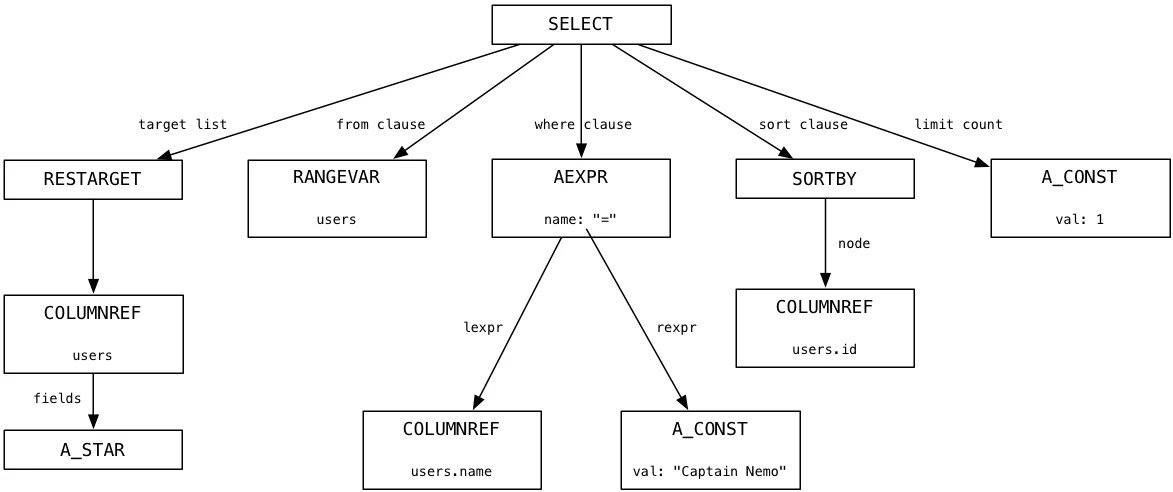
\includegraphics[width=\textwidth]{parse_tree.jpg}}
  \caption {Visualisation of parse tree for "SELECT * FROM users WHERE name = 'Captain Nemo' ORDER BY id ASC LIMIT 1'}
\end{figure}

\chapter{Existing options}
\section{Database libraries for Scala}
When we are working with databases in Java, we are most likely using JDBC, either directly or by wrappers like JPA or Hibernate. JDBC is available in Scala as well, by simply importing the \texttt{java.sql} API, you can create connections similarly as you would do in Java. But there are multiple existing libraries made for Scala, that ensure an easier way for the programmer to work with databases. Below I describe few selected libraries that were created for that specific reason.


\subsection{Quill}
Quill provides a Quoted Domain Specific Language (QDSL).~\cite{Quill} Its primary usage is to generate SQL queries, using only Scala code. Doing it this way Quill also provides type-safe queries, based on validation against defined database structure. The disadvantage of this approach is that the user can't validate generic queries without creating the case class database structure beforehand.

\subsection{Doobie}
Next up there is have Doobie, which is presented as \textit{"Doobie is a pure functional JDBC layer for Scala"}.~\cite{Doobie} In this library you can actually create pure SQL queries. The disadvantage is you have to have existing database and establish connection with it. That only allows run-time validation of queries.

\chapter{Realisation}

\section{Getting the SQL parse tree}
Since we want our library to work with parse trees of the SQL queries, first question we have to ask is how to get the internal parse tree itself. According to the official documentation\cite{PostgreSQL documentation} the parse tree gets created during the "Parser stage". Fortunately there already exists project, which extracts the parse tree called \texttt{Libpg\_query}.

\subsection{Libpg\_query}
\texttt{Libpg\_query} is an open-source C library created by Lukas Frittl. It uses the PostgreSQL server to access the internal \texttt{raw\_parse} function, which returns the internal parse tree. A minor disadvantage of this approach is that it uses the server code directly and it has to be compiled before it can be used. Then it accesses internal functions of the server which allows the library to get the parse tree for each valid query.

The main purpose of \texttt{libpg\_query} is to be used as a base library for implementations in other languages. There already exist multiple wrappers, for example \texttt{pg\_query} for Ruby or \texttt{pglast} for Python. However, at the moment of writing this thesis, there is no existing wrapper for it written for Scala. From \texttt{libpg\_query}, I am using the \texttt{pg\_query\_parse} function. Thanks to this function we can get the resulting parse tree in JSON format, which will be further processed by our Scala library.
\newpage
Here we have a simple code snippet describing simple usage taken from the GitHub README\cite{libpgquery}. 

\begin{lstlisting}[language=c]
#include <pg_query.h>
#include <stdio.h>

int main() {
  PgQueryParseResult result;
  result = pg_query_parse("SELECT 1");
  printf("%s\n", result.parse_tree);
  pg_query_free_parse_result(result);
}
\end{lstlisting}

\section{Parse tree representation in Scala}
Before we can start our work with the parse tree, it will prove useful to create our own structure, to represent that data in a form we can easily work with. 

The C library has its own struct representation for each type of possible Nodes that can be found in the internal PostgreSQL parse tree. That makes our job easier, because we just have to transform C structs to Scala case classes.

\bigskip
\newline
\textbf{Original C struct in \texttt{libpg\_query}}
\begin{lstlisting}[language=c]
    typedef struct A_Expr
    {
        NodeTag     type;
        A_Expr_Kind kind;
        List       *name; 
        Node       *lexpr; 
        Node       *rexpr; 
        int         location; 
    } A_Expr;
\end{lstlisting}
\bigskip
\textbf{Scala case class}
\begin{lstlisting}[language=scala]
    case class A_Expr(
        kind:     A_Expr_Kind.Value,
        name:     List[Node],
        lexpr:    Option[Node],
        rexpr:    Option[Node],
        location: Option[Int]
    ) extends Node
\end{lstlisting}


\section{Using native library}
Now we have a seemingly simple task to do. Just call the function from the \texttt{libpg\_query} library, which returns the parse tree in the form of JSON. Then we will convert the JSON into our case class structure. That is not as simple as it looks, and the reason for that is the conflict between native code and java byte code. 

\subsection{Native code and byte code}
Native code is compiled to run on a specific processor. Examples of languages that produce native code after compilation are C, C++. That means, every time we want to run our C program, it has to be recompiled for that specific operating system or processor.

Java byte code, on the other hand, is compiled source code from i.e. Java, Scala. Byte code is then translated to machine code using JVM. Any system that has JVM can run the byte code, does not matter which operating system it uses. That is why Java and Scala as well, are platform-independent.

Now because of this difference, we can't directly "import" the C library into our Scala code, but we have to use workaround, that enables this.

\subsection{Java native interface}
JNI is programming interface for writing Java native methods.\cite{JNI} It is used to enable Java code to use native applications and libraries. 

My earlier version of the project used JNI directly. I used \texttt{javah} command to generate C header file for \texttt{PgQueryWrapper}. The JNI C header file works as bridge between native code and Scala program. Now we can call libpg\_query inside the new C file, then compile it and create our shared library. Next step is loading the .so file into the Scala program. That was achieved by \texttt{System.loadLibrary} function. When that was done succesfully, we could finally receive the JSON containing the parse tree of our queries.

\subsection{sbt-jni}
Unfortunately, the preceding approach came with some problems. You had to modify the \texttt{java.library.path}, to add lib folder to it. When the project got separated into several subprojects, there was a problem with the system trying to use the shared library at the same time from different sources, which failed with \texttt{java.lang.UnsatisfiedLinkError} exception, since the native library was already loaded in different classloader. 

For thses reasons, I decided to use existing JNI wrapper for Scala called \texttt{sbt-jni}. It contains plugins to help working with native libraries, to name a few, JniJavah works as wrapper around the \texttt{javah} command to generate headers for classes with \texttt{@native methods}. Next one I used is JniLoad, which enables easy loading of shared libraries through \texttt{@nativeLoader} annotation.


\section{Parsing JSON result from libpg\_query}
There are few different libraries that can help with parsing JSONs. From those I decided to use \textit{circe}. Circe is fork of the pure functional library called Argonaut. It is great for parsing, traversing JSON, but the main functionality I used are the Encoders and Decoders. 

We have to generate Encoders and Decoders for every single case class, representing one of the nodes of the parse tree. 

\subsection{JSON structure}
Each node is in the JSON defined as key-value pair. Key is always the name of the node and value is dictionary where keys are names of the parameters with their corresponding values. 


\subsection{How decoding works}
Basic decoder for specific case class in \textit{circe} works as follows. JSON is parsed as key-value pairs and it attempts to map each parameter in case class to corresponding key from JSON. Return value from parsing is \texttt{Decoder.Result[T]}, which translates to \texttt{Either[DecodingFailure, T]}. As the name suggests, you get either \texttt{Left(DecodingFailure)} in case any invalid operation happens during the parsing, or \texttt{Right(T)}, where \texttt{T} is the required object that is supposed to be parsed. 

If the key is not found in the case class parameter list, it either sets the parameter to \texttt{None} (if the parameter is of \texttt{Option[T]} type), or returns \texttt{DecodingFailure}. If the value we are trying to further parse is not one of the built-in types, we have to implement Decoder for it. That means each of our case classes is required to have implementation of Decoder for everything to work smoothly.

\subsection{Using \texttt{circe}}
Input for parsing is always plain string representation of the query. \texttt{Libpg\_query} is then used to get the JSON representation of parse tree. Then I parse the JSON using \textit{circe} Decoder as Node type, which is an abstract class for all possible Nodes representing nodes of the SQL parse tree. In Node apply method correct Node subtype is chosen and Decoder for that subtype is used. Following the approach \textit{circe} uses, the parsing returns \texttt{Either[PgQueryError, Node]}.

\subsection{Parse expressions}
For parsing expressions, I use similar approach. The difference is that before the expression is sent to \texttt{libpg\_query}, the prefix "SELECT " is added. That way valid query should be created (if expression is valid) and following that the process is the same as for query. However, when we receive Node result, we have to get the expression only. That is done using pattern matching, since we expect \texttt{SelectStmt} node and we know its structure. Extracted expression is then returned as result.

\subsection{Prettify}
Prettify goes one step beyond the parsing of the query. In case the parse tree is built succesfully, it uses \texttt{Node.query} method. Depending on the structure of each Node, the query method is implemented to recursively build the whole parse tree back to SQL query in the string form.


\section{Scala custom interpolators}
\subsection{What are interpolators?}
Since version 2.10, Scala offers a new possibility of string interpolation.~\cite{String interpolation} This allows me to create generic queries with variables instead of direct values. That way we can define and reuse queries, without unnecessary copying and pasting of code. The idea behind Scala interpolation is the processing of string literals. For example, this code  \verb|id"Interpolated text"| is transformed into the call of method "id" on instance of \texttt{StringContext} class. By extending this existing class we can introduce custom interpolators, which allows for a clear definition of these generic query definitions.
\bigskip
\newline
\textbf{String concatenation}
\begin{lstlisting}[language=scala, showstringspaces=false]
val query: String = 
 "SELECT " + columnName + " FROM students WHERE " + expression
PgQueryParser.parse(query)
\end{lstlisting}
\bigskip
\textbf{String interpolation}
\begin{lstlisting}[language=scala, showstringspaces=false]
query"SELECT $columnName FROM students WHERE $expression"
\end{lstlisting}

\subsection{Implementation}
The first version of the library used only runtime validation. I defined my custom interpolator called \textit{query}

\subsection{`query` and `expr`}
There are currently two custom interpolators, one is meant for full, valid SQL queries, i.e. \texttt{SELECT * FROM students}. The second one is used for expressions, that can be inserted into the queries as parameters. Expression can be many different things, column name, constant, expression, function call etc.

\section{Scala macros}
Since we want to achieve compile time validation, we have to explicitly tell the Scala compiler. If the query would be defined as function, taking parameters, it would wait for runtime, when the parameters will be known (not just the types, as it is when compiling). And then each call to the function would be evaluated separately.

What we want to do is to validate query at compilation, so it creates at the parameter positions "placeholders". These will know the expected type, so every value passed to the function with matching type will result in valid query. In case the query is not valid, we will get compile time error right away, making it easier for us to debug the code and fix it.

That is where Scala macros are useful. They have same signature as functions, but their body consists of \texttt{macro} keyword and name of the macro function.  \textit{It will expand that application by invoking the corresponding macro implementation method, with the abstract-syntax trees of the argument expressions args as arguments.}~\cite{Def macros} I think that little description of what abstract syntax trees are is required here. In context of Scala, the AST is used as internal representation of the executed program. 

\subsection{Scala AST and Reflection library}
Macros are part of the Scala reflection library. We will specifically talk about the "Compile-time reflection". \textit{Scala reflection enables a form of metaprogramming which makes it possible for programs to modify themselves at compile time.}\cite{Compile-time reflection} 

When we enter execution of macro, we have the context and the function arguments. Everything is in the form of AST, so programming macros is slightly different from the usual programming in Scala. In simple terms context tells us where the macro was called from, which class, method name etc. 

\begin{figure}[h]
  \makebox[\textwidth]{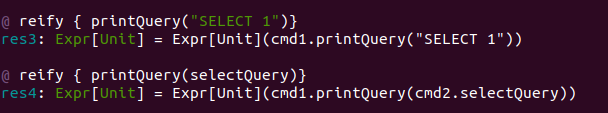
\includegraphics[width=\textwidth]{reify.png}}
  \caption {Differences in AST between parsing string directly and parsing variable}
\end{figure}

\subsection{Implementation}

\subsection{Lifting}

\section{Combining interpolators and macros}
\subsection{Parameterized queries in PostgreSQL}
Before we can get to the part, where our custom interpolator is simple call to the macro, which does the validation, we have to talk about implementation of placeholders in PostgreSQL. There is existing support for something called \textit{Prepared statements}. These allow for placeholders inside the query, in form of \textbf{\$n} where \textbf{n} must be positive integer.  

During compile time each variable in our interpolated string is during known by name only. In macro first thing we have to do is build the string itself from the \textit{StringContext} and the arguments. To keep the final query valid, each of the arguments has to be replaced with \textit{\$n}. 
Let's say we have the following example.
\begin{lstlisting}[language=scala, showstringspaces=false]
query"SELECT $columnName FROM students WHERE $expression"
\end{lstlisting}
If we tried to pass this string directly to the libpg\_query, we would get empty JSON result, because this is not a valid query. That means it is neccessary for us to transform it into this form.
\begin{lstlisting}[language=scala, showstringspaces=false]
query"SELECT $1 FROM students WHERE $2"
\end{lstlisting}
This returns correct parse tree, where each of the placeholders contains node of ParamRef type. 


\subsection{Transforming syntax tree}

\section{Testing}
\section{Summary}

\section{Publishing library}

\chapter{Conclusion}


\bibliographystyle{iso690}
\bibliography{mybibliographyfile}
\begin{thebibliography}{9}

\bibitem{PostgreSQL}
\textit {What Is PostgreSQL?} [online]. [cit. 2021-06-14]. Available from:
https://www.postgresql.org/docs/13/intro-whatis.html

\bibitem{Stackoverflow survey}
\textit {Stack Overflow Annual Developer Survey} [online]. [cit. 2021-06-13]. Available from: https://insights.stackoverflow.com/survey/2020\#technology-databases-all-respondents4

\bibitem{Quill} 
\textit {What is Quill?} [online]. [cit. 2021-04-25]. Available from: https://github.com/getquill/quill/
\bibitem{Doobie}
NORRIS, Rob. 
\textit {Doobie documentation} [online]. [cit. 2021-04-25]. Available from: https://tpolecat.github.io/doobie/
\bibitem{PostgreSQL documentation}
The PostgreSQL Global Development Group
\textit{The Parser Stage} [online]. [cit. 2021-06-20]. Available from: https://www.postgresql.org/docs/10/parser-stage.html
\bibitem{libpgquery}
FITTL, Lukas.
\textit {libpg\_query} [online]. [cit. 2021-04-25]. Available from:
https://github.com/pganalyze/libpg\_query

\bibitem{JNI}
Oracle
\textit{Java Native Interface} [online]. [cit. 2021-06-20]. Available from:
https://docs.oracle.com/javase/8/docs/technotes/guides/jni/

\bibitem{String interpolation}
SUERETH, Josh. 
\textit {String interpolation} [online]. [cit. 2021-04-25]. Available from: https://docs.scala-lang.org/overviews/core/string-interpolation.html
\bibitem{Def macros}
BURMAKO, Eugene. 
\textit {Def macros} [online]. [cit. 2021-04-25]. Available from: https://docs.scala-lang.org/overviews/macros/overview.html
\bibitem{Compile-time reflection}
Heather Miller, Eugene Burmako, Philipp Haller
\textit {Compile-time reflection} [online]. [cit. 2021-06-19]. Available from: https://docs.scala-lang.org/overviews/reflection/overview.html\#compile-time-reflection

\end{thebibliography}
\setsecnumdepth{all}
\appendix

\chapter{Acronyms}
% \printglossaries
\begin{description}
	\item[API] Application programming interface
	\item[JVM] Java virtual machine
	\item[JSON] JavaScript Object Notation
\end{description}


\chapter{Contents of enclosed CD}

%change appropriately

\begin{figure}
	\dirtree{%
		.1 readme.txt\DTcomment{the file with CD contents description}.
		.1 exe\DTcomment{the directory with executables}.
		.1 src\DTcomment{the directory of source codes}.
		.2 wbdcm\DTcomment{implementation sources}.
		.2 thesis\DTcomment{the directory of \LaTeX{} source codes of the thesis}.
		.1 text\DTcomment{the thesis text directory}.
		.2 thesis.pdf\DTcomment{the thesis text in PDF format}.
		.2 thesis.ps\DTcomment{the thesis text in PS format}.
	}
\end{figure}

\end{document}
